\section{Propylene}
%%
\subsection{Overview}
%------------------------------
\begin{frame}{Propylene architecture}
  %%
  \begin{itemize}
  \item Propylene is made of several \red{modules}
  \end{itemize}
  %%
  \begin{figure}[!h]
    \begin{center}
      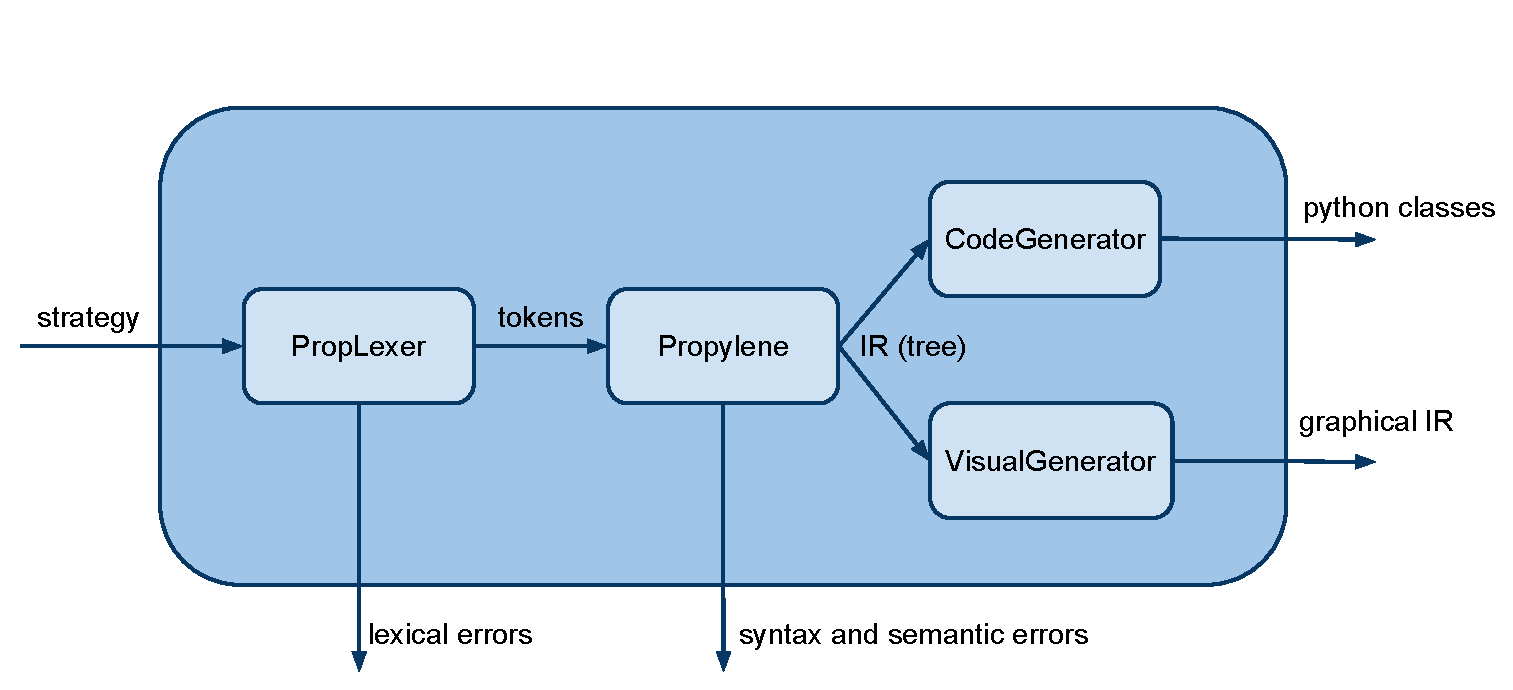
\includegraphics[width=300pt]{img/propylene.pdf}
    \end{center}
  \end{figure}
  %%
\end{frame}
%%
%%
%%
\subsection{PropLexer}
%------------------------------
\begin{frame}[fragile]{PropLexer}
  %%
  \begin{itemize}
  \item As the name suggests, it implements a {\bf lexer}
    \begin{itemize}
    \item takes as input a {\bf strategy}
    \item handles {\bf unexpected tokens}
    \item produces a stream {\bf tokens}
      \begin{itemize}
      \item a token can be requested via the \red{\texttt{token()}} method
      \end{itemize}
      \n
    \item makes use of {\bf conditional lexing}
      \begin{itemize}
      \item to distinguish between the same tokens in different \emph{contexts}
      \end{itemize}
    \end{itemize}
  \end{itemize}
  %%
  \begin{exampleblock}{Code snippet}
\begin{verbatim}
def t_STRING(self, t):
    r' " (\. | [^\\"])* " '
    return t
\end{verbatim}
  \end{exampleblock}  
  %%
\end{frame}
%%
%%
%%
\subsection{Propylene}
%------------------------------
\begin{frame}[fragile]{Propylene}
  %%
  \begin{itemize}
  \item It is the main module, implements a {\bf parser}
    \begin{itemize}
    \item takes as input the tokens produced by {\bf PropLexer}
    \item constructs and mantains a stack of {\bf symbol tables}
    \item handles {\bf syntax} and {\bf semantic} errors
    \item makes the {\bf parse tree}
    \item returns an {\bf intermediate representation} of the strategy
    \end{itemize}
  \end{itemize}
  %%
  \begin{exampleblock}{Code snippet}
\begin{verbatim}
def p_belief(self, p):
    ''' Belief  : NAME '(' ArgumentList ')'
    '''
    p[0] = Belief(uName=p[1])
    try: self.insert_symbol(p[1],'Belief')
    except AttitudeTypeMismatch as e:
        e.lineno = p.lineno(1)
        raise e
\end{verbatim}
  \end{exampleblock}  
  %%
\end{frame}
%%
%%
\subsection{The Intermediate Representation}
%------------------------------
\begin{frame}[fragile]{The Intermediate Representation (IR)}
  \begin{itemize}
  \item Similar to a \emph{decorated} parse tree
    \begin{itemize}
    \item some regions have been \emph{flattened}
    \end{itemize}
    \N
  \item Nodes are objects with an \red{\texttt{Accept (uVisitor)}} method to allow traversal
    \N
  \item An IR can be passed to either 
    \begin{itemize}
    \item the {\bf CodeGenerator} to generate \emph{python classes}
    \item the {\bf VisualGenerator} to generate a graphical representation of the IR
      itself
    \end{itemize}
  \end{itemize}
%%
\end{frame}
%%
%%
\begin{frame}[fragile]{An Example}
  \begin{exampleblock}{C.I.C.C.I.O. Strategy (Eurobot 2011)}
\begin{verbatim}
  ( +start() | (color("red")) ) >> 
                [ activate_poller(RedPathActivities),
                  activate_poller(KingQueenPoller),
                  activate_poller(TargetPoller) ]
\end{verbatim}
  \end{exampleblock}
  %%
  \begin{figure}[!h]
    \begin{center}
      \fbox{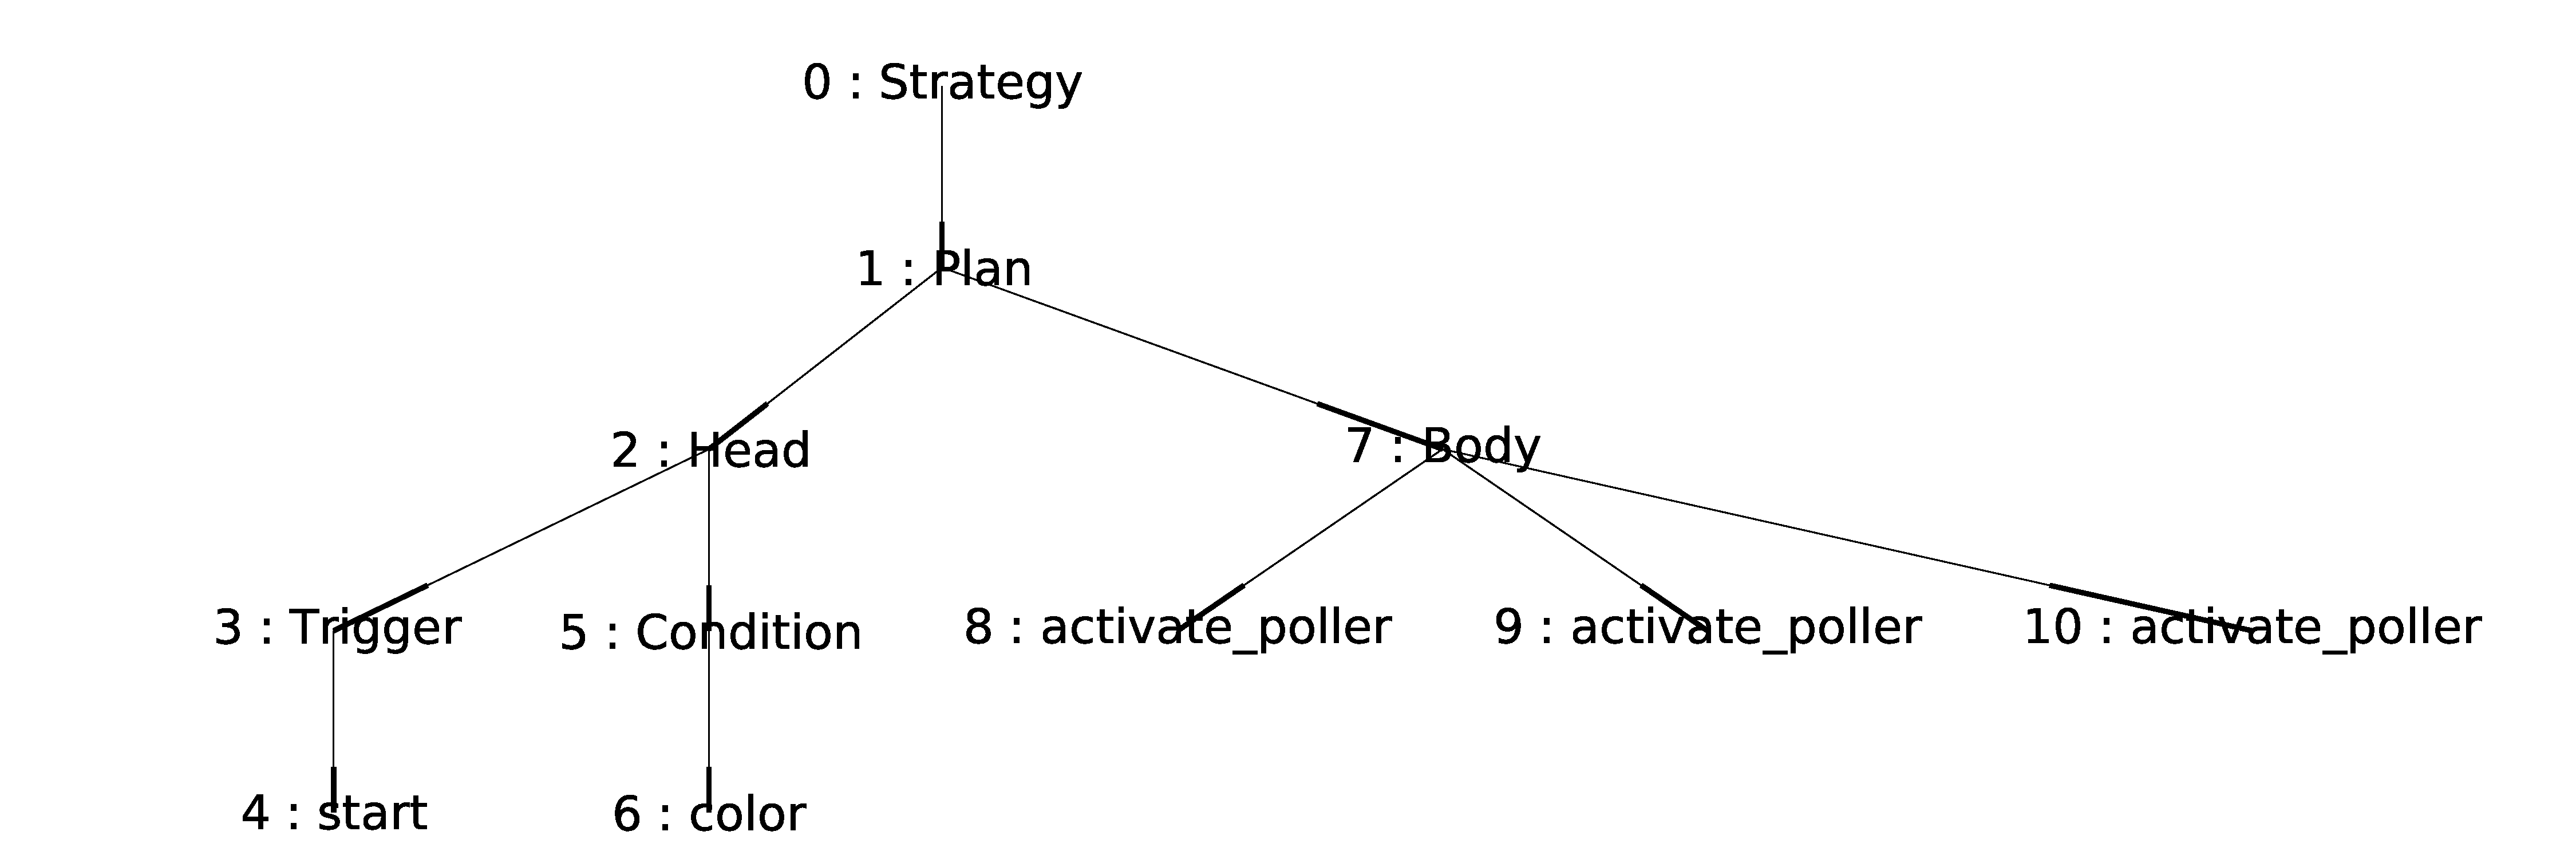
\includegraphics[width=300pt]{img/strategy-ir.pdf}}
    \end{center}
  \end{figure}
  %%
\end{frame}



\subsection{Error Handling}
%------------------------------
\begin{frame}[fragile]{Syntax Errors}
  %
  \begin{itemize}
    \item \navy{Propylene} attempts to recover from erroneous input 
    by using its error rules
\n
    \item When the encountered syntax errors exceed a threshold, 
    the parser stop
\n
    \item The user will be notified with info related to all errors
    
  \end{itemize}
  %
\N
%%
  \begin{exampleblock}{Error Messages Example}
\begin{verbatim}
Line 14: Syntax error - unexpected token `)'
Line 14: Illegal Triggering Event
Line 17: Error detected in the Condition of the plan
Line 96: Error detected in the Body of the plan
\end{verbatim}
  \end{exampleblock}
%%
%
\N\N
\end{frame}


%------------------------------
\begin{frame}[fragile]{Semantic Errors}
  %
  \begin{itemize}
    \item \navy{Propylene} is able to identify two types of semantic errors:
\n
  %
  \begin{enumerate}
    \item Unbounded Variable \\
\n
    %%
    \texttt {
        ( +\tildett deposit\_corns() | ( white\_corn(\_("Y")))) >>\\ 
        \tab [ +\tildett grab\_corn(\_("X")) \#ERROR! ]
            }
    %%
\N
    \item Attitude Type Mismatch \\
\n
    %%
    \texttt {
        ( +\tildett deposit\_corns() ) >>\\ 
            \tab [ +\tildett grab\_corn("c11") \\
            \tab \tab deposit\_corns() \#ERROR! ]
            }
    %%

  \end{enumerate}
  %
\n
  \item In both cases, the parser stops immediately and notifies the user
  about the encountered error
  \end{itemize}
  %
%
\N\N
\end{frame}


\subsection{Graphics}
%------------------------------
\begin{frame}{Graphics}
  %
  \begin{itemize}
    \item Tree graphics, diagrams
\N
    \item final remarks
%\N
%    \item 
%\N
%    \item
% 
  \end{itemize}
  %
%
\N\N
\end{frame}







%\subsection{}
%%------------------------------
%\begin{frame}{}
%  %
%  \begin{itemize}
%    \item
%\N
%    \item
%\N
%    \item 
%\N
%    \item
% 
%  \end{itemize}
%  %
%%
%\N\N
%\end{frame}


